\documentclass{article}
\usepackage{parskip}
\usepackage{pdfpages}
\usepackage{hyperref}
\usepackage{amsmath}
\usepackage[margin=.6in]{geometry}
\begin{document}
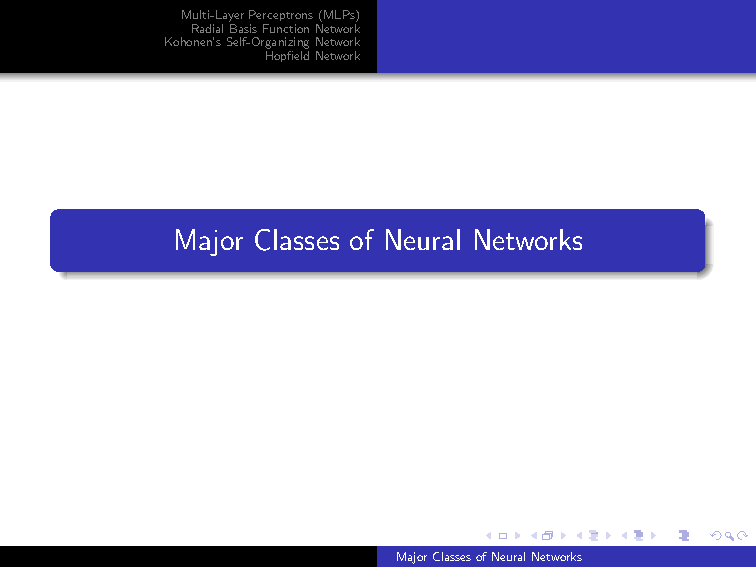
\includepdf[pages=1-6]{slides}
This is the struture of the neural network. It is the most general structure. An input layer is where signals enter the system. These are usually the features of an object. The yellow circles are just units. We call them perceptrons, this is a bit misleading. These perceptrons are different from the ones we saw earlier. The earlier ones create discrete values but they instead (most of the time) they have a smooth, nonlinear activation function. Their activation functions are very differentiable. They have the same structure though. The output layer generates the actual output of the system.

\includepdf[pages=7-9]{slides}
The multilayer perceptron has many layers to propagate signals. Most of the time, these kinds of models are supervised (we have to teach them).

This is still an optimization problem. We have some weights that we want to optimize our weights so that they have the least error. These kinds of systems have a ton of dimensions to optimize across. There will be very complex structures which make it very hard to actually solve. This is why we tend towards using other systems to get an optima even if its not the global optima.

When a solution is found (weights are known) we use this to find the weights of the next layer. This backpropagates the error signal through the layers backwards untill it reaches the first layer. You keep feeling in training signals until you run out and update all the weights. At this point we have finished one epoch.

Say you have $\overrightarrow{x}(x_1, ..., x_m)$ then you have the output $\overrightarrow{y}(y_1, ..., y_l)$ so we then get the mapping $\overrightarrow{y} = f(\overrightarrow{x})$. So your first training signal has to be a bunch of mappings of x to y. Roughly k signals.

\includepdf[pages=10]{slides}
Here $i$ is the index of the element we are looking at and $k$ is the index of the training set we are currently looking at. This makes an error function. We compute the sum of the square error for each node and propagate it backwards. We keep going backwards until we reach the communication layer (one right after the input layer).
\includepdf[pages=11]{slides}
\includepdf[pages=12]{slides}
Here is the update function for the weights. It looks pretty standard. We work layer by layer.

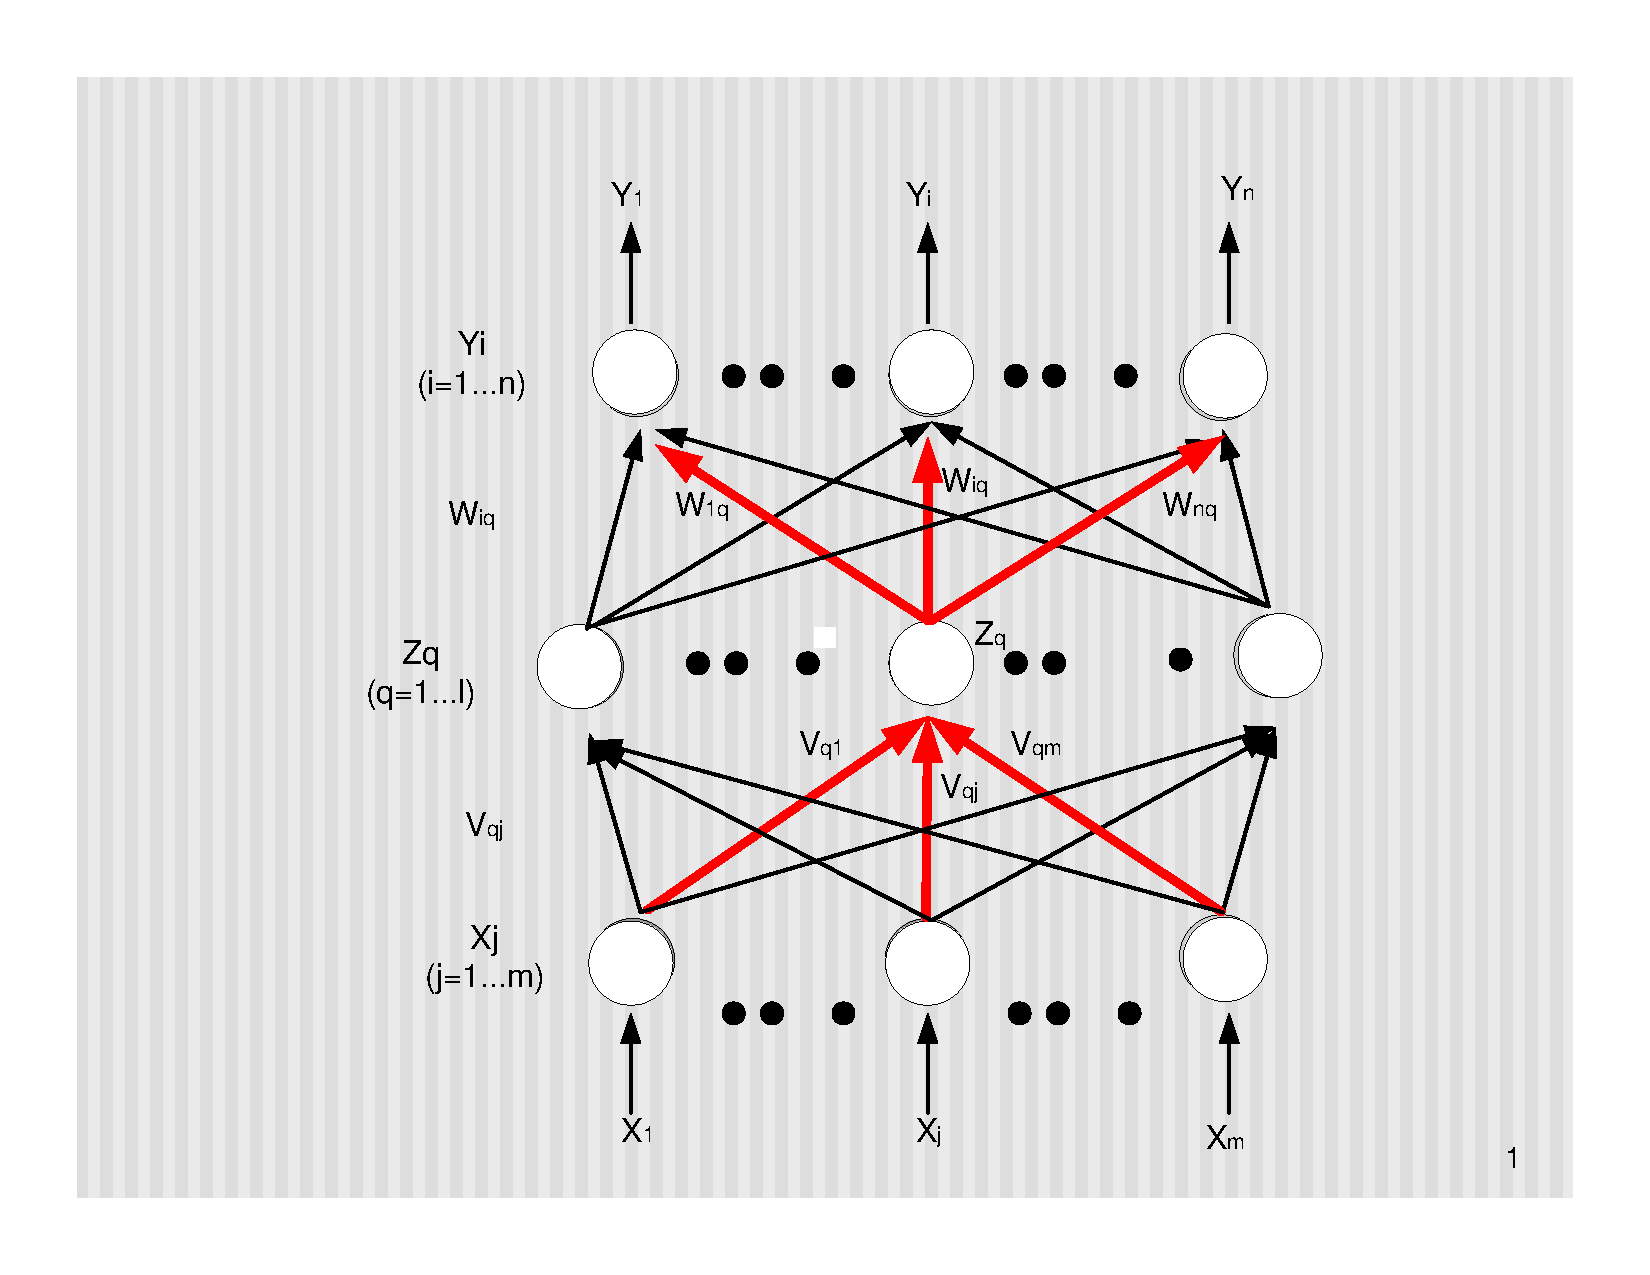
\includepdf[pages=1]{additional}
Here we have input layer $x$ with $m$ nodes in it, middle layer $z$ with $l$ nodes in it, and output layer $y$ with $n$ nodes in it. There are three weights going between $x$ and $z$ labeled with $v$, there are other ones but we are going to ignore them for simplicity in this example. There are other weights from $z$ to $y$ labeled as $w$, again there are others that we are just ignoring to make the example easier to go through. The subscript on the notation is the destination node,origin node notation. So how do we find the weights?

\begin{align*}
	a &= \text{activation function}\\
	net_q &= \sum_{j=1}^n v_{qj}x_j\\
	z_q &= a(net_q)\\
	&= a(\sum_{j=1}^n v_{qj}x_j)\\
	net_i &= \sum_{q=1}^l w_{iq}z_q\\
	y_i&= a(net_i)\\
	y_i &= a(\sum_{q=1}^l w_{iq}z_q)\\
	y_i &= a(\sum_{q=1}^l w_{iq}a(\sum_{j=1}^n v_{qj}x_j))\\
\end{align*}
In this case the two a functions do not have to be the same but its much easier if they are.

What about the target data (denoted $d_i$)?
\begin{align*}
	E &= \frac{1}{2}\sum_{i=1}^n(d_i - y_i)^2\\
\end{align*}

Remember we want gradient decay that eventually minimizes the error, after all this is an optimization problem.

Now we need to find our update functions for the shit ton of weights we have:
\begin{align*}
	\Delta w_{iq} &= -\eta\nabla_{w_{iq}} E(w)\\
	&= -\eta\frac{\delta E}{\delta w_{iq}}\\
	&= -\eta\frac{\delta E}{\delta y_{i}}\frac{\delta y_i}{\delta net_i} \frac{\delta net_i}{\delta w_{iq}}\\
	&= \eta(d_i - y_i)a'(net_i) z_q\\
	&= \eta\delta_{oi}z_q\\
	\delta_{oi}&= (d_i - y_i)a'(net_i)\\
	\Delta v_{qj} &= -\eta\nabla_{v_{qj}} E(w)\\
	&= -\eta\frac{\delta E}{\delta v_{qj}}\\
	&= -\eta\frac{\delta E}{\delta net_q}\frac{\delta net_q}{\delta v_{qj}}\\
	&= -\eta\frac{\delta E}{\delta z_q}\frac{\delta z_q}{\delta net_q}\frac{\delta net_q}{\delta v_{qj}}\\
	&= \eta\sum_{i=1}^{n}\left ((d_i - y_i)a''(net_i)w_{iq} \right )a'(net_q)x_j\\
	&= \eta \delta_{hq}x_j\\
	\delta_{hq} &= a'(net_q) \sum_{i=1}^n \delta_{oi}w_{iq}
\end{align*}
This is the output for only one hidden layer, more work is required for more layers.

We snag E and keep it constant though all the layers and let it run until E updates with a new training signal. So the E value should be the same through out all the udpates.

To see the full slide of this:

\includepdf[pages=2-4]{additional}

\includepdf[pages=5-6]{additional}
Now lets say we have an arbitrary number of layers $Q$, so the $z$ layer in the previous example becomes ${}^{q-1}y$ and the $y$ layer becomes ${}^qy$.

The tolerance error is the max error we will allow. We know it will never reach 0 so we instead give it a threshold to work for. Something that is good enough.

\includepdf[pages=7]{additional}
Step 1: apply your first set of data. Starting at the top layer (where $q+1$).

Step 2: propagate the signal forward. Keep calculating the output  of each layer until  you get to the end.

Step 3: calculate the error of the system. The error equation shows two Es. This one being added at the time is the previous error, so its cumulative.

\includepdf[pages=8]{additional}
Step 4: propagate the error signal back. Here we are just updating our weights as we go.

Step 5: just cycle through a nice epoch

Step 6: check if your error is low enough. cycle if not

steps 5 and 6 are basically the same looping conditions of the adeline system.

\includepdf[pages=18-19]{slides}

\includepdf[pages=11-17]{slides}
$\Delta w^L = \delta^L x^{L-1}$ This is the relationship between layers. These will propagate backwards untill it reaches the input.

\begin{align*}
	\Delta w_{ij}^L &= \eta \left[ t_i - o_i^L \right] f'(tot)_i^L o_J^{L-1}\\
	f(tot)_i^L &= \frac{\delta f(tot)^L}{\delta tot_i^L}\\
	\delta_i^L &= \text{Error of the system}\\
\end{align*}

Here $f$ is the sigmoid function $f(x) = \frac{1}{1+e^{-x}}$. We like this activation function because it is infinitely differentiable $\frac{\delta f}{\delta x} = f(1-f)$. This is almost universally used.

\begin{align*}
	\Delta w_{ig}^L &= \eta \delta_i^L o_j^{L-1}\\
	\delta_i^L &= (t_i - o_i^L)(o_i^L)(1-o_i^L)\\
\end{align*}


All of the above processes are online training. An alternative is batch/offline training where you put all of the input in at the same time. Usually online returns better results but there are places where offline training is helpful.

Now we look at propagating backwards: $l < L$
\begin{align*}
	\Delta w_{ij}^l &= \eta \delta^lo_j^{l-1}\\
	\delta_i^l &= f'(tot_i)^l \sum_{p=1}^{nl} \delta_p^{l+1}w_{pi}^{l+1}\\
	nl &= \text{number of hidden layers}\\
	\delta_i^l &= o_i^l(1-o_i^l)\sum_{p=1}^{nl} \delta_p^{l+1}w_{pi}^{l+1}\\
	\Delta w_{ij}^l &= \eta o_i^l(1-o_i^l) \sum_{p=1}^{nl} \delta_p^{l+1}w_{pi}^{l+1}
\end{align*}
These equations areht emost equations used in back propagation.

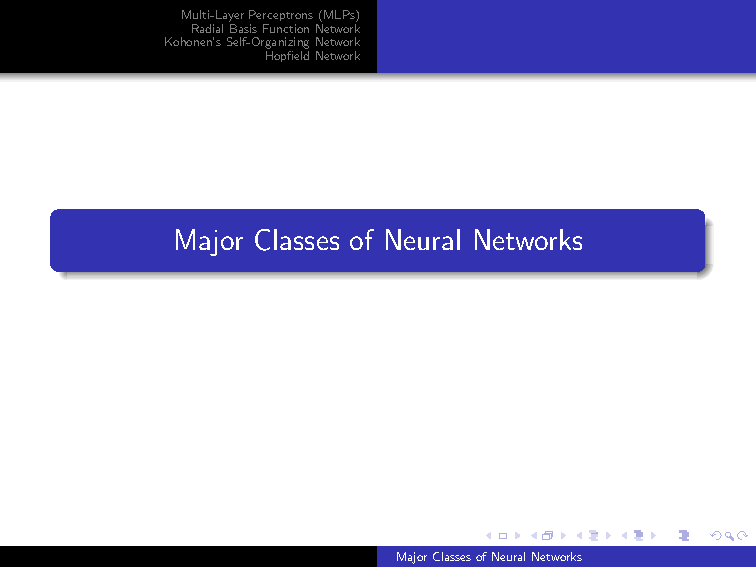
\includepdf[page=20-21]{slides}
Momentum helps us from oscillating like crazy, and encourages convergence.

So now we update our weights with the learning curve times the gradient descent plus some constant times the previous value of delta omega. This gives the system a bit of memory. It is now improving on earlier values of weight. The gradient descent is still small when compared to the previous value of omega. This means that delta omega is going to be very close to its previous value.

This method is very commonly used.

Bellow is an example, he chose not to go over it in class. In this example the bias is kept separate from the terms. This way it can be injected at certain areas. Remember that it is not always there. We see here that the output is scalar which is a bit new. Nothing really changes though.

Remember, you refresh the error between epochs. This is called online learning. Online learning has a smaller memory footprint than batch learning.

NOTE: this will likely be an example of a kind of question that could be on the exam. know it.

There are some typos:
\begin{itemize}
	\item slide 29, lowest line should be $\delta_6 = $ the rest of the line
\end{itemize}


\includepdf[pages=22-35]{slides}


Now we have a system with three nodes
\includepdf[pages=36-39]{slides}
We can accidentally have too many nodes, we say that this causes the system to be \textbf{overtrained}. We do lots of cross validation, data changing, and reconfiguring of the system to see which form converges best. Basically you use a bunch of data to tune the system before you apply the testing data.
\includepdf[pages=39-41]{slides}
The more varied your training data the better your system, but the more nodes you have might not improve things.

\includepdf[pages=43]{slides}
\includepdf[pages=44]{slides}
\includepdf[pages=45]{slides}
If the system is not converging you have to reshuffle your data or the structure of your network.

NOTE: know how the different configurations and values can effect the system.

Below is another example he didnt go through
\includepdf[pages=46-51]{slides}

Now lets look at topology
\includepdf[pages=52-53]{slides}
The typical activation for an MLP is tanh or sigmoid since they are infinitely differentiable.

We now consider closed/bounded activation functions that start high and get lower (a bit like converging). The best for the following system is the Gausian membership function.

\includepdf[pages=54]{slides}
Here we have central nodes that have maximum results and the edges less so. Here we only have weights between the hidden layer and the output layers. You can think of this as the weights between the input layer and the hidden layer as one.

We dont want a system to pass between all of the points, we want to it interpolate between the points. This is usually the result of \textbf{overfeeding}.

When we get our data set we should separate it into training, validation, and testing sets. Training and validation is used to create a system that will try to predict properly the results of the testing data. We can shuffle the training and validation data around to hone in the right amount of training for the system. The training is the one that tunes up the weights. The validation is used to validate the model that you produced. Do not go to the testing part if the validation is not good.

The behavior of the system depends on:
\begin{itemize}
	\item the number of training data (you can control this)
	\begin{itemize}
		\item larger is better
	\end{itemize}
	\item architecture of the network, nodes and hidden layers (you can control this)
	\begin{itemize}
		\item a medium value is needed, gotta tune this
	\end{itemize}
	\item the behavior of the system or its linearity (you cannot control this)
\end{itemize}
this is probably going to be on the exam

The interpolator solution can create a very good approximation of your system even if it is nonlinear.

NOTE: I think his slides are borked again, so this might need syncing with them later

We can perfectly approximate a nonlinear function with an adequate number (that we need to find) if some other functions that we sum.

This is basically linear combination of bayes gaussian network. If you chose which of these functions you use your error can go to 0.

\includepdf[pages=55]{slides}
Here we are mapping a nonlinear function into higher dimensional domains. We want to extract from the system, all of the representatives of the overall system and cluster it into unique local systems.

\includepdf[pages=56]{slides}
From the input layer to the middle layer there is the unity value (weights are 1) which is a unique character to radial systems.

\includepdf[pages=57]{slides}
\includepdf[pages=58]{slides}
The generation of these functions required unsupervised learning. This is why it is called a hybrid system. One components is supervised and the other is through clustering.

We need the weights, the mean, and the standard deviations.

Weights are through supervised learning. The mean and standard deviation is through unsupervised learning.

\includepdf[pages=59]{slides}

Usually the center of the network has the same number of inputs as outputs.

So its the euclidean distance between the input vector and the center of the radial function, divided by some width parameter all of which fed into the activation function (I think r is the activation, needs to be confirmed).

\includepdf[pages=60]{slides}
both of these variations of g are used as possible functions. The first is far more common, but some situations use the second with justification.

\includepdf[pages=61]{slides}
We still consider $\omega$ as the weights between nodes.

The receptive field is another name for the radial function.

\includepdf[pages=62]{slides}
First we use an unsupervised training to get the center vector (aka mean) and a scalar for the spread (aka standard deviation). Then we do supervised training to get the weights.

\includepdf[pages=63]{slides}
\includepdf[pages=64]{slides}
\includepdf[pages=65]{slides}
For the interpolation problem the number of training data is equal to the hidden layer nodes. If you have 20 nodes you have 20 training data. Remember this, called \textbf{interpolation}.

\includepdf[pages=66]{slides}
\includepdf[pages=67]{slides}
D is the desired output and $G^{-1}$, if it exists, gives us the weights.

If $G^{-1}$ doesn't exists, it might be \textbf{illconditioned}. This happens if the determinant is very small resulting in large numbers. If this occurs it we use a non-square matrix.

This happens if the number of training data is not equal to the number of hidden nodes as well.
\includepdf[pages=69]{slides}
\includepdf[pages=70]{slides}
Suppose we have a function. We have 5 radial function, the center for each one at a training data. We have have an interpolation problem because we have the same number of inputs as training data.

\includepdf[pages=71]{slides}
here are the funcitons we will use.

The one on the right uses a randomly chosen spread of 0.5. This is clearly incorrect.

\includepdf[pages=72]{slides}
He we tried a different spread with much better results.

\includepdf[pages=73]{slides}
This one is overreaching on the spread.

It is important to extract this value from unsupervised training.
\includepdf[pages=74]{slides}
\includepdf[pages=75]{slides}
\includepdf[pages=76]{slides}

RBF has been proven to be better than the multilayer perceptron.

Having a single hidden layer is much better and easier to work with. Its more transparent.

Which speed is faster depends on the complexity of the problem. For simple problems MLP is faster but RBF is better for larger systems.


\includepdf[pages=77]{slides}
\includepdf[pages=78]{slides}
























\end{document}
